\documentclass[11pt]{article}
\usepackage[T1]{fontenc}
\usepackage{lmodern,microtype,amsmath,amssymb,amsthm,mathtools,booktabs,array,xurl}
\usepackage[a4paper,margin=28mm]{geometry}
\usepackage{tikz}
\usetikzlibrary{arrows.meta,calc,positioning}
\usepackage[colorlinks=true,linkcolor=blue!55!black,citecolor=blue!55!black,urlcolor=blue!55!black]{hyperref}
\numberwithin{equation}{section}
\setlength{\emergencystretch}{2em}
\newtheorem{theorem}{Theorem}[section]
\newtheorem{proposition}[theorem]{Proposition}
\newtheorem{lemma}[theorem]{Lemma}
\newtheorem{corollary}[theorem]{Corollary}
\theoremstyle{definition}\newtheorem{definition}[theorem]{Definition}
\theoremstyle{remark}\newtheorem{remark}[theorem]{Remark}
\newcommand{\ii}{\mathrm i}
\newcommand{\dd}{\mathrm d}
\newcommand{\CC}{\mathbb C}
\newcommand{\RR}{\mathbb R}
\newcommand{\Log}{\operatorname{Log}}
\newcommand{\tr}{\operatorname{tr}}
\newcommand{\diag}{\operatorname{diag}}
\newcommand{\Vol}{\operatorname{Vol}}
\title{Nonparabolic holonomy of trees of crossing circles}
\author{}\date{}
\begin{document}\maketitle
\begin{abstract}
We construct marked holonomy for an ordered tree of crossing circles
while allowing the main meridian to become nonparabolic.
An explicit two-octahedron chart gives all face maps, the two primitive
auxiliary similarities and a regular four-puncture character chart.
The disk-side shear ratios sew in the original page order. Retained
half twists require the full Hurwitz action on the puncture generators,
followed by a compatible choice of eigenflags.
At a positive primitive filling point the original augmented
triangulation supplies an unramified one-dimensional filled
representation germ. The proof keeps logarithmic filling marks and
distinguishes killing a slope word from merely setting its eigenvalue
ratio to one. No quantum asymptotic or preferred-longitude formula is
assumed.
\end{abstract}

\section{The original diagram and the statements}\label{ng:introduction}

A crossing circle bounds a disk punctured twice by the main strands.
We retain that disk, its framing, and the ordered endpoints of its
two-strand tangle. A finite tree $\mathcal T$ has at least one edge.
Each vertex has its own crossing-circle tangle; every tree edge is a
physical quarter-turn attachment of ordered stacks. There are no
product junctions without a crossing circle. Products, rotations,
endpoint frames and the cylindrical closing map are part of the
specified diagram. At circle $v$ retain a crossing
$R^{\epsilon_v}$ with $\epsilon_v\in\{-1,0,1\}$.
Assume that the main strands form one component, and orient it.
Write $Y^\epsilon$ for this original augmented link exterior in $S^3$.

The ordered cut of \cite[Proposition~2.1]{Circle} gives two projection
balls. Each edge contributes a pair of octahedra. Around a circle,
its disk-side pages occur in the original cyclic order; one
distinguished seam carries its retained half twist. This topological
result includes the inverse cut, the original peripheral paths and
the primitive crossing-circle basis. We use that specific cut,
not an arbitrary collection of algebraically matching octahedra.

The positive main meridian has determinant-one eigenvalues $M,M^{-1}$.
We select the $M^{-1}$ eigenline. The auxiliary disk longitude at
circle $v$ has selected eigenvalue $-Q_v$, and therefore projective
similarity $Q_v^2$ in the chart sending that flag to infinity.
A projective similarity means the dilation multiplier of an affine
map in this chart. It is the ratio of the selected eigenvalue to the
other one, not an unspecified primitive square root.

For each edge $e=vw$ introduce $X_e$ and impose
\begin{equation}\label{ng:T1}
 (X_e+Q_v)(X_e+Q_v^{-1})(X_e+Q_w)(X_e+Q_w^{-1})
 =(X_e-1)^2(1-X_eM^2)(1-X_e/M^2).
\end{equation}
The selected branch passes through $M=Q_v=1$, $X_e=\ii$.
Set
\begin{equation}\label{ng:T2}
 \rho_{v,e}=\frac{Q_v+X_e}{1+Q_vX_e},
 \qquad f_e=\frac{M^2-X_e}{1-M^2X_e}.
\end{equation}
All rational statements are on the open sets where their displayed
denominators are nonzero. They continue on the same irreducible
component; clearing a denominator does not add a geometric branch.

\begin{theorem}[The marked augmented representation]\label{ng:representation}
For each fixed ordered tree and retained half-twist pattern,
\eqref{ng:T1} constructs a holomorphic framed representation of the
original $\pi_1(Y^\epsilon)$ near its marked complete structure.
It uses the selected main eigenflag and the original primitive
auxiliary curves. Their similarity logarithms, centered at completeness,
are
\begin{equation}\label{ng:T3}
 U_v=\sum_{e\ni v}\log\rho_{v,e}-\epsilon_v\log Q_v,
 \qquad V_v=2\log Q_v .
\end{equation}
The family is the local decorated representation germ, modulo
simultaneous projective conjugation, with coordinates
$(\log M,(\log Q_v)_v)$.
Its actual ideal triangulation remains positive nearby.
The same construction and marking continue to the positive
circle-filling endpoints supplied by \cite[Theorem~1.1 or
Theorem~7.1]{Circle}.
\end{theorem}

Here a decorated representation retains a common fixed flag for each
peripheral subgroup and its exact eigenvalue character.
At a nonparabolic main cusp the structure is incomplete; the theorem
does not assert a complete metric there. The explicit character
matrices in Theorem~\ref{ng:character} also give rational full-group
identities away from the initial face-coordinate chart.

Fill circle $v$ along its original primitive slope
$\mu_v+p_v\lambda_v$, and put $n_v=\epsilon_v-2p_v$.
The surgery is the original disk twist: cutting the twice-punctured
disk, rotating through $p_v$ full turns and removing its circle inserts
$R^{n_v}$ in that same frame. It takes place in $S^3$.
Exponentiating the primitive slope equation gives
\begin{equation}\label{ng:T5}
             \prod_{e\ni v}\rho_{v,e}=Q_v^{n_v}.
\end{equation}

\begin{theorem}[The marked filled meridian germ]\label{ng:filled-germ}
Suppose an original primitive filling has a positive retained
augmented triangulation and its endpoint is the actual complete
filled holonomy. Suppose also that every filled auxiliary longitude
has distinct eigenvalues. Near that endpoint, imposing the continued
logarithmic equations
\begin{equation}\label{ng:A2}
                  U_v+p_vV_v=-2\pi\ii
\end{equation}
is exactly imposing the projective filled-group relations.
If there is one unfilled main cusp, the resulting decorated germ,
modulo simultaneous conjugation, is smooth and one-dimensional,
with coordinate $\log M$ and the prescribed $M^{-1}$ flag.

For the present trees these hypotheses hold whenever
$\sqrt{d_v^2+n_v^2}\ge630$ at every circle, where $d_v$ is its tree
degree, and also under the heterogeneous certificate of
\cite[Theorem~7.1]{Circle}. In these cases the germ is that of the
original filled knot exterior. Independently long signed powers
satisfy the first condition for every fixed tree. The theorem also
allows a small or zero power when the stated geometric criterion holds.
\end{theorem}

The first paragraph is a general local statement about an original
positive augmented triangulation. It does not require a newly added
subdivision to be positive, nor a positive ideal triangulation of the
filled manifold. This form permits its use with another independently
constructed positive anchor.

For $Q_v^2\ne1$, equation \eqref{ng:T5} makes the slope word
projectively identity, because it commutes with the semisimple
longitude. At $Q_v=\pm1$ that assertion fails in general:
a nontrivial parabolic matrix also has eigenvalue ratio one.
Likewise, an arbitrary exponentiated solution does not specify the
logarithmic mark \eqref{ng:A2} or prove metric completion.
Theorem~\ref{ng:filled-germ} retains the actual smooth endpoint.

The proofs below use three classical companion inputs:
the ordered cut and positive geometric anchors of \cite{Circle};
the original positive odd-meridian convention of
\cite[Section~5, equations~(5.1)--(5.2)]{Strict}; and the
normal-path row/intersection identity of
\cite[Section~7.1, equation~(7.2)]{Marked}.
The last input will be used only for the real gluing-row ranks and
polarization, not for any quantum source or longitude conclusion.
We prove the needed local rigidity on the retained triangulation.

\section{The local face maps}\label{ng:the-local-face-maps}

We first construct the two-octahedron piece with its original
white and shaded face labels. In this section \(E_0\) is a preliminary
white-face coordinate, and \(X\) is the edge variable in \eqref{ng:T1}.
Their distinction matters when \(M\ne1\).

\subsection{The parameters and the actual faces}\label{ng:the-parameters-and-the-actual-faces}

Write \(M\) for the main meridian eigenvalue parameter and set
\(m=M^2\). The symbols \(Q\) and \(P\) are the chosen square roots
of the two auxiliary longitude similarities. All parameters are near
\((m,Q,P)=(1,1,1)\). We use \(E_0\) for a white-face
coordinate, near \(i\). The meridian-determined wire coordinate will be
denoted \(X\).

The two projection copies have six ideal vertices

\begin{equation}\label{ng:N1}
\begin{array}{c|c|c}
 &\text{equator}&\text{circle apices}\\ \hline
 +&(0,\infty,1,R)&(A,B)\\
 -&(0,\infty,1,S)&(a,b).
 \end{array}
\end{equation}

The four white identifications are the unique maps of the ordered
triangles

\begin{equation}\label{ng:N2}
\begin{aligned}
 W_0:(A,0,\infty)&\longmapsto(a,0,\infty),&
 W_1:(B,\infty,1)&\longmapsto(b,\infty,1),\\
 W_2:(A,1,R)&\longmapsto(a,1,S),&
 W_3:(B,R,0)&\longmapsto(b,S,0).
\end{aligned}
\end{equation}

These are the face labels of the original two-leaf cut. Changing the
minus equator from \(R\) to \(S\) is necessary: retaining the old
four white matrices would keep all four main meridians parabolic.

Put \(L=E_0^{-1}\), and define

\begin{equation}\label{ng:N3}
\begin{gathered}
 S=\frac{m^2R}{1+(m^2-1)R},\qquad
 \ell_1=L/m,\quad \ell_2=L/m^2,\quad \ell_3=Lm,\\
 c_2=\frac{\ell_2(R-1)/(S-1)-1}{R-1},\qquad
 c_3=\frac{\ell_3R/S-1}{R},\\
 W_0=\begin{pmatrix}L&0\\0&1\end{pmatrix},\quad
 W_1=\begin{pmatrix}\ell_1&1-\ell_1\\0&1\end{pmatrix},\\
 W_2=\begin{pmatrix}c_2+\ell_2&1-c_2-\ell_2\\c_2&1-c_2\end{pmatrix},
 \qquad
 W_3=\begin{pmatrix}\ell_3&0\\c_3&1\end{pmatrix}.
\end{gathered}
\end{equation}

Thus \(W_2(z)=1+\ell_2(z-1)/(1+c_2(z-1))\).
Every map sends its two equatorial vertices in \eqref{ng:N2} correctly.

If \(q=(0,\infty,1,R)\), the native main corner word
\(W_{j-1}^{-1}W_j\) fixes \(q_j\) and has local derivative

\begin{equation}\label{ng:N4}
(m^{-1},m,m^{-1},m)_j.
\end{equation}

At infinity the local coordinate is \(1/z\). To derive \eqref{ng:N3},
start with \(W_0(z)=Lz\). The derivatives at infinity, 1 and 0
give respectively \(\ell_1=L/m,\ell_2=L/m^2,\ell_3=Lm\).
The remaining derivative at \(R\), on its branch through the
complete chart, gives the displayed formula for \(S\).
This supplies the actual peripheral condition, not just equal traces.

\subsection{The auxiliary longitude equations and the local gluing locus}\label{ng:the-auxiliary-longitude-equations-and-the-local-gluing-locus}

Take

\begin{equation}\label{ng:N5}
A=\frac{mE_0+Q}{m+Q},\qquad B=\frac{P(1-mE_0)}{P+m},\qquad
 a=A/E_0,\qquad b=1+\frac{B-1}{E_0m}=-\frac{B}{E_0P}.
\end{equation}

There are two expressions for the equatorial coordinate:

\begin{equation}\label{ng:N6}
\begin{aligned}
 R_v&=\frac{(mE_0+Q)(mE_0Q+1)}
 {E_0m(Q^2+1)+2E_0Qm^2+Q(1-m^2)},\\
 R_w&=-\frac{P(mE_0-1)^2}
 {E_0m^2(P^2+1)+2E_0Pm+P(m^2-1)}.
\end{aligned}
\end{equation}

The first is exactly \(W_2(A)=a\); the second is exactly
\(W_3(B)=b\). Their common value is \(R\).

For completeness, the longitude choices made here can be obtained
before solving for the apices. The first longitude is
\(W_2^{-1}W_0\). Its similarity in the coordinate with \(A\)
at infinity is \(W_2'(A)/L\), and is prescribed as \(Q^2\).
The chosen square-root branch is
\(1+c_2(A-1)=-1/(mQ)\). At the other circle the longitude is
\(W_1^{-1}W_3\), with similarity
\(\ell_1/W_3'(B)=P^2\), and the chosen branch is
\(1+c_3B=-mP\). Substitution gives \eqref{ng:N5}--\eqref{ng:N6}.
Both signs equal \(-1\) at completeness.

Clearing the nonzero denominators of \(R_v-R_w\), and removing
the factor \(E_0m^2\), gives

\begin{equation}\label{ng:N7}
\begin{aligned}
G={}&E_0^2P^2Qm^2+E_0^2PQ^2m+2E_0^2PQm^2+2E_0^2PQm
       +E_0^2Pm+E_0^2Qm^2\\
 &+E_0P^2Q^2m+E_0P^2m-4E_0PQm+E_0Q^2m+E_0m\\
 &+P^2Q+PQ^2m+2PQm+2PQ+Pm+Q.
\end{aligned}
\end{equation}

The local gluing equation is \(G=0\). At \(m=Q=P=1\),
\(G=8(E_0^2+1)\), so \(G_{E_0}(i,1,1,1)=16i\).
It follows that there is a unique holomorphic branch \(E_0\) near
\(i\). Every denominator displayed above is nonzero on a sufficiently
small neighborhood of this branch.

The pure shaded maps in the two plus-copy circle frames are

\begin{equation}\label{ng:N8}
S_v(A,R)=
 \begin{pmatrix}0&RA(1-A)\\A-R&R-A^2\end{pmatrix},\qquad
 S_w(B,R)=
 \begin{pmatrix}B(B-1)&-RB(B-1)\\B-R&R-B\end{pmatrix}.
\end{equation}

The first fixes \(A\) and sends \(\infty\) to \(0\) and \(1\)
to \(R\). The second fixes \(B\) and sends \(R\) to \(0\)
and \(1\) to infinity. The minus maps are the same formulas with
\((A,B,R)\) replaced by \((a,b,S)\); denote them by
\(S_v^-\) and \(S_w^-\).

All the actual white/shaded edge returns hold projectively:

\begin{equation}\label{ng:N9}
\begin{array}{lll}
 W_0S_v=S_v^-W_0,&W_2S_v=S_v^-W_2,&W_3S_v=S_v^-W_1,\\
 W_1S_w=S_w^-W_1,&W_3S_w=S_w^-W_3,&W_0S_w=S_w^-W_2.
\end{array}
\end{equation}

The first row follows already on \(R=R_v\), and the second on
\(R=R_w\). One can verify each equality by multiplying one side
by the adjugate of the other: both off-diagonal entries and the
diagonal difference vanish. Consequently these are the face maps
of the marked local representation of the original cut, rather than
maps chosen solely to reproduce a character polynomial.

At completeness their apices are

\begin{equation}\label{ng:N10}
(A,B)=((1+i)/2,(1-i)/2),\quad
 (a,b)=((1-i)/2,(1+i)/2),\quad R=S=1/2.
\end{equation}

Use the original apical subdivision and positive quad orders of
\cite[Lemma~3.1]{Circle}. Its eight ordered tetrahedral shapes
are then \(i\). Holomorphic continuity preserves their
positive imaginary parts on a sufficiently small parameter
neighborhood. This is a local incomplete hyperbolic structure with
decorated main eigenflags; it does not assert completeness at a
nonparabolic main cusp.

\subsection{The wire coordinate is determined by the actual meridian}\label{ng:the-wire-coordinate-is-determined-by-the-actual-meridian}

The positively chosen auxiliary meridians are \(S_v^{-1}\) and
\(S_w^{-1}\). Sending the corresponding apex to infinity changes
their similarities into the ordinary derivatives of \(S_v,S_w\)
at those apices. Direct differentiation of \eqref{ng:N8} gives

\begin{equation}\label{ng:N11}
\begin{aligned}
 U_v^{\exp}
 &=-\frac{A(A-R)}{R(1-A)}
   =\frac{(E_0m+Q)(Qm+1)}{(Q+m)(E_0Qm+1)},\\
 U_w^{\exp}
 &=\frac{B(R-1)}{(B-R)(B-1)}
   =\frac{(E_0+P)(P+m)}{(E_0P+1)(Pm+1)}.
\end{aligned}
\end{equation}

These are similarities of the primitive words, not the squares of
unrecorded primitive words. The actual longitude similarities are
exactly \(Q^2,P^2\), as established in Section~\ref{ng:the-auxiliary-longitude-equations-and-the-local-gluing-locus}.

Solve \(U_v^{\exp}=(Q+X)/(1+QX)\) for \(X\).
Cancel the removable \(Q=1\) factor before taking that limit:

\begin{equation}\label{ng:N12}
X=
 \frac{E_0Q^2m+E_0Qm^2+E_0Qm+E_0m-Qm+Q}
 {E_0Qm^2-E_0Qm+Q^2m+Qm+Q+m}.
\end{equation}

The denominator is \(4\) at completeness. The second meridian
similarly gives

\begin{equation}\label{ng:N13}
X_w=-\frac{E_0P^2m+E_0Pm+E_0P+E_0m+Pm-P}
 {E_0Pm-E_0P-P^2-Pm-P-1}.
\end{equation}

Their difference is \((m-1)G\) divided by the product of the
two displayed denominators. Hence \(X=X_w\) on the actual
gluing locus. In particular

\begin{equation}\label{ng:N14}
U_v^{\exp}=\frac{Q+X}{1+QX},\qquad
 U_w^{\exp}=\frac{P+X}{1+PX},\qquad X|_{m=1}=E_0.
\end{equation}

Thus the same source wire variable is selected from both actual
auxiliary meridians.

Substitution of \eqref{ng:N12} and \eqref{ng:N7} now gives

\begin{equation}\label{ng:N15}
(X+Q)(X+Q^{-1})(X+P)(X+P^{-1})
       =(X-1)^2(1-Xm)(1-X/m).
\end{equation}

For a direct polynomial check, after reducing the rational
expression its numerator is \(G\) times
\[
 (Q+1)^2(Q+m)(Qm+1)
       (E_0Q^2m+E_0Qm^2+E_0Qm+E_0m-Qm+Q).
\]
Nonzero unit factors can differ if the common denominator is not
reduced. Alternatively put
\(\mathcal A=X+X^{-1}\), \(\mathcal B=Q+Q^{-1}\),
\(\mathcal C=P+P^{-1}\), \(\mathcal D=m+m^{-1}\).
Equation \eqref{ng:N15} is

\begin{equation}\label{ng:N16}
(\mathcal A+\mathcal B)(\mathcal A+\mathcal C)
  =(\mathcal A-2)(\mathcal A-\mathcal D),\qquad
 \mathcal A=\frac{2\mathcal D-\mathcal B\mathcal C}
                  {\mathcal B+\mathcal C+\mathcal D+2}.
\end{equation}

The denominator in the last expression is \(8\) at completeness.
This is the effective edge equation with \(m=M^2\).

\subsection{The full disk-side seam, including its main punctures}\label{ng:the-full-disk-side-seam-including-its-main-punctures}

Use the ordered cross ratio
\([a,b,c,d]=(a-c)(b-d)/((a-d)(b-c))\).
The incoming plus-copy triangle at the first circle is
\((A,\infty,1)\); the outgoing triangle is \((A,R,0)\).
Develop the adjacent minus triangle back through its actual white
map. The six neighboring third vertices are respectively

\begin{equation}\label{ng:N17}
E_0,\quad W_1^{-1}(a),\quad W_2^{-1}(\infty),\qquad
 W_2^{-1}(0),\quad W_3^{-1}(a),\quad W_0^{-1}(S).
\end{equation}

Substituting \eqref{ng:N3}--\eqref{ng:N6}, with \(R=R_v\), gives

\begin{equation}\label{ng:N18}
\begin{array}{c|ccc}
 \text{incoming edge}&(A,\infty)&(\infty,1)&(1,A)\\ \hline
 \text{ratio}&-m/Q&-Q&-1/(mQ)\\
 \text{outgoing edge}&(A,R)&(R,0)&(0,A)\\ \hline
 \text{ratio}&-mQ&-1/Q&-Q/m .
\end{array}
\end{equation}

For example, the first ratio is \((A-1)/(A-E_0)=-m/Q\).
The other five reduce by the same single substitution. In particular
the table is independent of the other circle parameter \(P\) and
of the preliminary wire coordinate \(E_0\).

The original pure disk-side matching reverses the two main
punctures: outgoing \((A,R,0)\) is identified with incoming
\((A',1,\infty)\). Thus the outgoing entries are paired with
the incoming entries in reverse order. Each resulting product is
one, including its complex shear. A map of the three ordered
vertices identifies the first triangles; the three ratios then
identify the adjacent second triangles. This proves equality of
the full marked two-triangle disk-side structures. It does not
replace that matching by an arbitrary pants permutation.

The main puncture multipliers visible in the incoming table are
\(m,m^{-1}\), and the circle multiplier is \(Q^{-2}\);
the outgoing table reverses the boundary orientation. These
multipliers explain why recording the puncture order is essential.
Replacing \(M\) by \(M^{-1}\) exchanges eigenflags and is not
an innocuous reset of the marked representation.

Consequently any chain of these \emph{compatibly framed pure seams}
can be sewn in its original cyclic order. The geometric seam at
each step uses the same \(m,Q\); it requires no parameter from
the opposite end of an edge. Products of the auxiliary meridian
increments are therefore products of the factors in \eqref{ng:N14}.
The actual main component and its globally positive meridian
must still be traced through the endpoint frames, as explained
in Section~\ref{ng:ordered-pages-and-the-half-twist-collar} below.

\section{A regular character chart for the same piece}\label{ng:a-regular-character-chart-for-the-same-piece}

The face chart identifies the actual topology. The following rational
matrix chart is useful both for its peripheral words and for continuation
to generic auxiliary values over any fixed \(M\ne0\).
Throughout this section use

\begin{equation}\label{ng:C0}
\begin{gathered}
 t=M+M^{-1},\quad D=M^2+M^{-2}=t^2-2,\\
 \beta=Q+Q^{-1},\quad\gamma=P+P^{-1},\\
 A_0=X+X^{-1},\quad S=\beta+\gamma+t^2.
 \end{gathered}
\end{equation}

Equation \eqref{ng:T1} is

\begin{equation}\label{ng:C0a}
(A_0+\beta)(A_0+\gamma)=(A_0-2)(A_0-D),\qquad
 A_0=\frac{2D-\beta\gamma}{S}.
\end{equation}

The denominator is eight at completeness. In the following matrix
formulas the internal mixed trace is denoted \(\mathcal X\), so it
is distinct from the source wire \(X\).

\begin{theorem}[The local character and its marking]\label{ng:character}
The matrices constructed in this section give a determinant-one
four-puncture representation and invertible projective auxiliary
transports on their displayed regular open set of \eqref{ng:T1}.
Their full two-generator conjugacy identities, primitive auxiliary
ratios and local main commutator are rational identities there.
Near the complete point they are conjugate, with the indicated
selected flags and original peripheral words, to the actual face
representation of Section~\ref{ng:the-local-face-maps}.
\end{theorem}

We prove the statement by constructing the matrices and then matching
all their words to the native cut.

\subsection{A four-puncture character and its explicit matrices}\label{ng:a-four-puncture-character-and-its-explicit-matrices}

Put

\begin{equation}\label{ng:C5}
p=-\beta,\qquad q=-\gamma,\qquad \mathcal X=2+SX,
 \qquad b=p-2,\quad h=M-M^{-1}.
\end{equation}

For the moment \(p,q,\mathcal X\) may be arbitrary nearby parameters. Define

\begin{equation}\label{ng:C6}
A=\begin{pmatrix}M&1\\0&M^{-1}\end{pmatrix},
 \qquad
 B=\begin{pmatrix}M^{-1}&0\\b&M\end{pmatrix}.
\end{equation}

Both have determinant one and trace \(t\), and \(\operatorname{tr}(AB)=p\). Set

\begin{equation}\label{ng:C7}
\begin{gathered}
 c=\frac{M\mathcal X+M^{-1}q-2t}{D-p},\qquad
 d=\frac{q-M^2-1+hc}{p-2},\\
 e=\mathcal X-1-M^{-2}-hc,\qquad
 C=\begin{pmatrix}c&d\\e&t-c\end{pmatrix}.
 \end{gathered}
\end{equation}

The denominators \(p-2=-4\) and \(D-p=4\) at the complete point are nonzero. The construction does not divide by \(M-M^{-1}\). Direct multiplication gives

\begin{equation}\label{ng:C8}
\operatorname{tr}C=t,\qquad
 \operatorname{tr}(BC)=q,\qquad
 \operatorname{tr}(AC)=\mathcal X,\qquad
 \operatorname{tr}(ABC)=t.
\end{equation}

For the last identity, the nonconstant part of the trace is
\(bc+Me+M^{-1}bd\), which vanishes by \eqref{ng:C7}.

The determinant calculation is

\begin{equation}\label{ng:C9}
\det C-1=\frac{\mathcal F(\mathcal X,p,q)}{(p-2)(D-p)},
\end{equation}

where

\begin{equation}\label{ng:C10}
\mathcal F=
 \mathcal X^2+p^2+q^2+pq\mathcal X-2t^2(p+q+\mathcal X)+4t^2+t^4-4.
\end{equation}

This is the equal-boundary-trace four-punctured-sphere character equation, derived here from the matrices. For a direct verification of \eqref{ng:C9}, substitute the three entries in \eqref{ng:C7}, multiply by \((p-2)(D-p)\), and collect the quadratic polynomial in \(\mathcal X\). Its leading coefficient is one; the other two coefficients are those displayed in \eqref{ng:C10}.

Now impose \eqref{ng:C5}. A direct substitution gives the especially simple identity

\begin{equation}\label{ng:C11}
\mathcal F(2+SX,-\beta,-\gamma)
 =XS\bigl[(A_0+\beta)(A_0+\gamma)
                         -(A_0-2)(A_0-D)\bigr].
\end{equation}

Thus \eqref{ng:T1} is equivalent to \(\det C=1\) on this regular chart. Put

\begin{equation}\label{ng:C12}
D_0=(ABC)^{-1}.
\end{equation}

Equations \eqref{ng:C8}--\eqref{ng:C12} give

\begin{equation}\label{ng:C13}
ABCD_0=I,\qquad
 \det A=\det B=\det C=\det D_0=1,\qquad
 \operatorname{tr}A=\operatorname{tr}B
       =\operatorname{tr}C=\operatorname{tr}D_0=t.
\end{equation}

These are literal matrices representing the four positively oriented boundary generators of a four-punctured sphere. Each puncture has eigenvalues \(M,M^{-1}\). In particular, the source relation is not merely similar in degree to a character equation: \eqref{ng:C7}, \eqref{ng:C11}, and \eqref{ng:C12} realize it by actual matrices.

At the complete selected point,

\begin{equation}\label{ng:C14}
A=\begin{pmatrix}1&1\\0&1\end{pmatrix},\quad
 B=\begin{pmatrix}1&0\\-4&1\end{pmatrix},\quad
 C=\begin{pmatrix}-1+2i&1\\8i&3-2i\end{pmatrix}.
\end{equation}

All four punctures are noncentral parabolics. The pair \(A,B\) has no common eigenline. The construction is therefore on a regular irreducible character chart through the complete point.

The alternative root of the quadratic \eqref{ng:C10} is \(2+S/X\). Indeed its sum with \(\mathcal X=2+SX\) is \(2t^2-\beta\gamma\), by \eqref{ng:C0a}. For comparison, its discriminant factors as

\begin{equation}\label{ng:C15}
(\beta+2)(\gamma+2)
       \bigl[\beta\gamma-2\beta-2\gamma-4D-4\bigr]
           =S^2(X-X^{-1})^2.
\end{equation}

This verifies the two-sheeted parameter and its branch without assigning signs by a numerical square root.

\subsection{Auxiliary transport matrices with the actual source ratios}\label{ng:auxiliary-transport-matrices-with-the-actual-source-ratios}

Define two invertible projective transport matrices

\begin{equation}\label{ng:C16}
V=AB+z_v I,\qquad T=BC+z_w I,
 \qquad
 z_v=-\frac{1+X(\beta+1)}{1-X},\qquad
 z_w=\frac{X+\gamma+1}{1-X}.
\end{equation}

Scalar multiples of \(V,T\) give the same projective transports. Their determinant-one normalizations can be chosen on a local square-root cover; every commutator below is independent of that choice.

The following full matrix identities hold on \eqref{ng:T1}:

\begin{equation}\label{ng:C17}
\begin{aligned}
 VA&=D_0^{-1}V,& VB&=C^{-1}V,\\
 TB&=A^{-1}T,& TC&=D_0^{-1}T.
 \end{aligned}
\end{equation}

They are stronger than trace matching. Also \(V\) commutes with \(AB\), and \(T\) commutes with \(BC\), directly from \eqref{ng:C16}.

Here is a rational way to verify \eqref{ng:C17}, preserving the regular chart. Eliminate \(\gamma\) using \eqref{ng:C0a}:

\begin{equation}\label{ng:C18}
\gamma=\frac{2D-(X+X^{-1})(\beta+D+2)}
                         {X+X^{-1}+\beta}.
\end{equation}

The denominator is two at the complete point. Substitute \eqref{ng:C18}, \eqref{ng:C5}, and \eqref{ng:C7} in \eqref{ng:C17}. Every difference becomes a zero rational function of \(M,\beta,X\). This is also a polynomial certificate after clearing the recorded denominators. For example, before substituting \eqref{ng:C5}, the value of \(z\) solving the lower-left entry of
\((AB+zI)A=(ABC)(AB+zI)\) makes the remaining three entries scalar multiples of \eqref{ng:C10}; after \eqref{ng:C5}, that \(z\) reduces to \(z_v\). The other pair follows by cyclic permutation of the four punctures. No eigenline diagonalization at a repeated eigenvalue is used.

The two disk-longitude words and their selected eigenvalues are

\begin{equation}\label{ng:C19}
\Lambda_v=AB,\quad \lambda_v=-Q;
 \qquad
 \Lambda_w=(BC)^{-1},\quad \lambda_w=-P.
\end{equation}

The inverse in the second word records the opposite boundary orientation. On the \(-Q\) eigenline of \(AB\), the projective eigenvalue ratio of \(V\) is

\begin{equation}\label{ng:C20}
\frac{z_v-Q}{z_v-Q^{-1}}
                         =\frac{Q+X}{1+QX}.
\end{equation}

This identity follows by factoring the numerator as
\(-(1+Q)(1+X/Q)/(1-X)\) and the denominator as
\(-(1+Q^{-1})(1+XQ)/(1-X)\).

For \(T\), note \(z_w=z_v(P,X^{-1})\). Its ratio on the \(-P\) eigenline of \(BC\) is therefore the inverse of \((P+X)/(1+PX)\). The selected eigenline of \(\Lambda_w=(BC)^{-1}\) with eigenvalue \(-P\) is instead the \(-P^{-1}\) eigenline of \(BC\). Thus its marked ratio is

\begin{equation}\label{ng:C21}
\frac{z_w-P^{-1}}{z_w-P}
                         =\frac{P+X}{1+PX}.
\end{equation}

Equations \eqref{ng:C20}--\eqref{ng:C21} are exactly the two source auxiliary ratios. Their extension to \(Q=P=1\) is the full matrix limit of \eqref{ng:C16}, not a separate evaluation of two coalescing eigenvectors.

The determinants are nonzero nearby. More explicitly, after \eqref{ng:C18},

\begin{equation}\label{ng:C22}
\begin{aligned}
 \det V&=\frac{(\beta+2)(\beta X+X^2+1)}{(X-1)^2},\\
 \det T&=
 -\frac{(X-1)^2(X-M^2)(XM^2-1)
                (\beta M^2+M^4+1)}
 {M^4(\beta X+X^2+1)^2}.
 \end{aligned}
\end{equation}

Both equal \(-4\) at the complete point. These formulas fix the regularity needed for the inverse transport matrices.

\subsection{The main commutator gives the source longitude factor}\label{ng:the-main-commutator-gives-the-source-longitude-factor}

Consider the ordered commutator

\begin{equation}\label{ng:C23}
\Lambda_K=T V^{-1}T^{-1}V.
\end{equation}

It commutes with \(A\). This also follows from the transport paths: its inverse \(V^{-1}TVT^{-1}\) sends \(A\) successively to \(B^{-1}\), \(C\), \(D_0^{-1}\), and back to \(A\), using \eqref{ng:C17}.

Set

\begin{equation}\label{ng:C24}
u=\frac{M^2-X}{1-M^2X}.
\end{equation}

The exact matrix is

\begin{equation}\label{ng:C25}
\Lambda_K=
 \begin{pmatrix}
 -u & (u^{-1}-u)/(M-M^{-1})\\
 0  & -u^{-1}
 \end{pmatrix}.
\end{equation}

The apparent quotient in its upper-right entry is removable at \(M=1\). A direct certificate, without multiplying four complicated inverse matrices, is

\begin{equation}\label{ng:C26}
T V=V
 \begin{pmatrix}
 -u^{-1}&(u-u^{-1})/(M-M^{-1})\\
 0&-u
 \end{pmatrix}T.
\end{equation}

Substitution of \eqref{ng:C7}, \eqref{ng:C16}, and \eqref{ng:C18} makes every entry of the difference zero. Multiplication by \(V^{-1}\) and \(T^{-1}\), which are legitimate by \eqref{ng:C22}, gives \eqref{ng:C25}. The expression for the upper-right entry is regular because \(u=1\) at \(M=1\).

The \(M\) eigenline of the positively oriented puncture \(A\) is the first coordinate line. Thus the eigenvalue of \eqref{ng:C23} on that line is \(-u\), exactly the source factor for one edge. The original source cut selects the opposite \(M^{-1}\) eigenline; its eigenvalue is \(-u^{-1}\), retaining the required inverse-flag convention.

Write \(X=e^{2\pi i x}\), using the logarithm selected by \(x=1/4\)
at the complete edge. At \(M=1\), with \(X\) kept on its continued branch,

\begin{equation}\label{ng:C27}
\Lambda_K=
 \begin{pmatrix}
 -1&-2i\cot(\pi x)\\0&-1
 \end{pmatrix}.
\end{equation}

Since \(A\) translates by one, \eqref{ng:C27} has projective translation
\(2i\cot(\pi x)\). At the complete edge \(x=1/4\), this is \(2i\).
The negative determinant-one lift in \eqref{ng:C25} is the actual commutator lift; it was not inserted by multiplying the word by a sign. No global preferred-longitude formula follows from this local calculation alone.

\subsection{Comparison with the explicit native pure block}\label{ng:comparison-with-the-explicit-native-pure-block}

The face construction in Section~\ref{ng:the-local-face-maps} supplies the geometric marking
for these character matrices. The comparison retains the original
white-map order and all six white/shaded returns. Section~\ref{ng:ordered-pages-and-the-half-twist-collar} then
assembles the ordered tree and its odd seams.

Write its four actual white maps as \(W_0,W_1,W_2,W_3\), and its two plus-copy shaded maps as \(S_v,S_w\). The equatorial corners are \(0,\infty,1,R\). Put

\begin{equation}\label{ng:C28}
N_j=W_{j-1}^{-1}W_j,\qquad j\bmod4.
\end{equation}

The native corner maps have derivatives
\((M^{-2},M^2,M^{-2},M^2)\) in the finite local coordinates, with \(1/z\) at infinity. They obey
\(N_0N_1N_2N_3=I\) by literal cancellation of the white maps.

In the matrix representatives fixed in that construction,

\begin{equation}\label{ng:C29}
\det W_0=L,\quad \det W_1=L/M^2,\quad
 \det W_2=L/M^4,\quad \det W_3=LM^2.
\end{equation}

The determinant-one puncture matrices to compare with \eqref{ng:C6}--\eqref{ng:C13} are therefore

\begin{equation}\label{ng:C30}
A_{\mathrm g}=M^{-3}N_3,\quad
 B_{\mathrm g}=MN_0,\quad
 C_{\mathrm g}=MN_1,\quad
 D_{\mathrm g}=MN_2.
\end{equation}

Their product is one, since the four displayed scalar powers multiply to one. Each trace is \(M+M^{-1}\): its eigenvalue ratio is prescribed by the native corner derivative, its determinant is one, and its trace tends to \(2\) at completeness. Thus the sign is fixed by continuity, rather than reset on a puncture independently.

The two disk words now agree with their actual geometric words, including their determinant-one lifts:

\begin{equation}\label{ng:C31}
A_{\mathrm g}B_{\mathrm g}=M^{-2}W_2^{-1}W_0,\qquad
 (B_{\mathrm g}C_{\mathrm g})^{-1}
                         =M^{-2}W_1^{-1}W_3.
\end{equation}

These are the native \(v,w\) longitudes. Their selected eigenvalues are \(-Q,-P\), with their actual apex flags. The inverse in the second abstract word is essential to \eqref{ng:C31}.

\subsubsection{Actual auxiliary transports and character normalization}\label{ng:actual-auxiliary-transports-and-character-normalization}

The native shaded paths send the corners as follows:

\begin{equation}\label{ng:C32}
S_v:\infty\mapsto0,\quad 1\mapsto R;\qquad
 S_w:R\mapsto0,\quad 1\mapsto\infty.
\end{equation}

Their six white/shaded return identities imply, for the native punctures, that these paths reverse the oriented small boundary meridian at each endpoint. Thus

\begin{equation}\label{ng:C33}
\begin{aligned}
 S_vC_{\mathrm g}S_v^{-1}&=B_{\mathrm g}^{-1},
 &S_vD_{\mathrm g}S_v^{-1}&=A_{\mathrm g}^{-1},\\
 S_wA_{\mathrm g}S_w^{-1}&=B_{\mathrm g}^{-1},
 &S_wD_{\mathrm g}S_w^{-1}&=C_{\mathrm g}^{-1}.
 \end{aligned}
\end{equation}

For example, the projective relation \(W_3S_v\sim S_v^-W_1\), together with
\(W_0S_v\sim S_v^-W_0\), gives
\[
 S_v(W_0^{-1}W_1)S_v^{-1}\sim W_0^{-1}W_3=N_0^{-1}.
\]
The native matrix representatives can differ by a nonconstant scalar in this calculation; those scalars are not set to one. Normalize the punctures using \eqref{ng:C30}. The two sides now have determinant one and trace \(t\), so their projective equality has scalar \(+1\), since \(t\ne0\) near completeness. The remaining three identities follow from the other returns in the same way. This proves the literal determinant-one identities \eqref{ng:C33} without discarding a projective scalar.

Consequently

\begin{equation}\label{ng:C34}
V_{\mathrm g}=S_v^{-1},\qquad
                       T_{\mathrm g}=S_w^{-1}
\end{equation}

satisfy exactly \eqref{ng:C17}. These are the actual positively marked auxiliary meridians of the native construction, not extra operators inserted into the tangle.

There is a regular marked conjugacy to the character coordinates. At completeness the selected \(M\)-eigenlines of \(A_{\mathrm g},B_{\mathrm g}\) are distinct. Their eigenlines vary holomorphically: the matrices minus their specified eigenvalue have rank one with a nonzero entry near the parabolic point. Send those two eigenlines to infinity and zero, then fix the residual diagonal conjugation by setting the upper-right entry of \(A\) to one. This entry is a unit near completeness. The pair becomes exactly \eqref{ng:C6}, since \(\operatorname{tr}(AB)=-\beta\) fixes \(b=-\beta-2\).

The remaining matrix \(C\) is then determined by its trace, the two mixed traces, and \(\operatorname{tr}(ABC)=t\), giving \eqref{ng:C7}. The common centralizer of this irreducible pair consists only of scalars. Hence a transport satisfying \eqref{ng:C17} is unique projectively: the ratio of two such transports commutes with both punctures. Its marked eigenvalue ratio is therefore \eqref{ng:C20}, not a new free parameter.

The branch is fixed by the literal complete matrices. Substituting the complete native white maps gives
\(A_{\mathrm g}=\left(\begin{smallmatrix}3-2i&-1+i\\4-4i&-1+2i\end{smallmatrix}\right)\)
and
\(C_{\mathrm g}=\left(\begin{smallmatrix}1&-1+i\\0&1\end{smallmatrix}\right)\).
Their product has trace \(2+8i\). Since \(S=8\), the character coordinate \((\operatorname{tr}(A_{\mathrm g}C_{\mathrm g})-2)/S\) is \(i\), not the inverse root.

Let \(X_{\mathrm g}\) denote the native source wire extracted from its actual auxiliary meridian:

\begin{equation}\label{ng:C35}
U_v^{\exp}=\frac{Q+X_{\mathrm g}}{1+QX_{\mathrm g}}.
\end{equation}

The character coordinate \(X\) has the same ratio by \eqref{ng:C20}. For \(Q^2\ne1\), the fractional-linear map in \eqref{ng:C35} is injective, so \(X=X_{\mathrm g}\). Holomorphic continuation establishes equality through \(Q=1\). Equivalently,

\begin{equation}\label{ng:C36}
\operatorname{tr}(A_{\mathrm g}C_{\mathrm g})
       =2+\bigl[\beta+\gamma+(M+M^{-1})^2\bigr]X_{\mathrm g}.
\end{equation}

This proves the matching branch, rather than choosing the inverse root because the two have the same discriminant.

\subsubsection{Main basepoint, selected flag, and negative lift}\label{ng:main-basepoint-selected-flag-and-negative-lift}

The native geometric longitude based at infinity is

\begin{equation}\label{ng:C37}
\Lambda_\infty=S_wS_v^{-1}S_w^{-1}S_v.
\end{equation}

Its positively oriented main meridian is \(C_{\mathrm g}=MN_1\). In the native chart it is exactly

\begin{equation}\label{ng:C38}
C_{\mathrm g}=
 \begin{pmatrix}
 M^{-1}&M E_0-M^{-1}\\0&M
 \end{pmatrix},
\end{equation}

where \(E_0\) is the native white-face coordinate. Thus infinity is its actual \(M^{-1}\) source flag. The white-face coordinate \(E_0\) need not equal the source coordinate \(X=X_{\mathrm g}\) away from \(M=1\).

Our abstract commutator is based at the corner \(R\), whose positive meridian is \(A_{\mathrm g}\). The actual path

\begin{equation}\label{ng:C39}
U=S_w^{-1}S_v,\qquad
 \infty\longrightarrow 0\longrightarrow R.
\end{equation}

transports both the meridian and longitude:

\begin{equation}\label{ng:C40}
UC_{\mathrm g}U^{-1}=A_{\mathrm g},\qquad
 U\Lambda_\infty U^{-1}
      =S_w^{-1}S_vS_wS_v^{-1}
      =T_{\mathrm g}V_{\mathrm g}^{-1}
                         T_{\mathrm g}^{-1}V_{\mathrm g}.
\end{equation}

The first identity follows from \eqref{ng:C33}, including its two inversions; the second is literal multiplication of the four words. The source \(M^{-1}\) eigenflag is transported by this same path. It is not identified with infinity in the normalized matrix \eqref{ng:C6}, where infinity is instead the \(M\) eigenline.

Equations \eqref{ng:C25}, \eqref{ng:C36}, and \eqref{ng:C40} identify the native longitude eigenvalues exactly: on its source \(M^{-1}\) eigenflag the value is \(-u^{-1}\); on the preferred \(M\) flag it is \(-u\). The negative sign survives the basepoint change. At completeness the native matrix is

\begin{equation}\label{ng:C41}
\Lambda_\infty=
 \begin{pmatrix}-1&2+2i\\0&-1\end{pmatrix},\qquad
 C_{\mathrm g}=
 \begin{pmatrix}1&i-1\\0&1\end{pmatrix}.
\end{equation}

Their projective translations have ratio \(2i\), equal to \eqref{ng:C27}. This checks the actual marked complete lift and scale; it is not the reason for the full rational identification above.

Thus the two constructions agree on the canonical pure block, its main eigenvalue, its two primitive auxiliary words, and the lift of this local main word. This proves Theorem~\ref{ng:character}. The next section assembles the ordered tree. Identifying a globally preferred main longitude is a separate framing question.

\section{Ordered pages and the half-twist collar}\label{ng:ordered-pages-and-the-half-twist-collar}

At the second end of an edge, in the same native face notation,
the incoming triangle is \((B,R,1)\) and the outgoing triangle
is \((B,\infty,0)\). Their neighboring third vertices are

\begin{equation}\label{ng:S0}
W_3^{-1}(1),\ W_2^{-1}(b),\ W_1^{-1}(S),\qquad
 W_1^{-1}(0),\ W_0^{-1}(b),\ W_3^{-1}(\infty).
\end{equation}

Substitution gives the tables

\begin{equation}\label{ng:S0a}
I(m^{-1},P)=(-1/(Pm),-P,-m/P),\qquad
 O(m^{-1},P)=(-P/m,-1/P,-Pm).
\end{equation}

At the first end use \(I(m,Q),O(m,Q)\) from \eqref{ng:N18}.
The original reversed triangle matching pairs outgoing entries with
the incoming entries in reverse order, and every product is one.
Thus both the angles and the complex shears match.

\subsection{An arbitrary finite pure page tree}\label{ng:an-arbitrary-finite-pure-page-tree}

Let the original tree have no retained odd seam. Choose one
bipartition sign \(\sigma_v\in\{1,-1\}\), so adjacent
vertices have opposite signs. At an edge with first endpoint
\(v\), use the local chart with \(m_e=m^{\sigma_v}\).
Its other endpoint then has parameter \(m^{\sigma_w}\) by
\eqref{ng:S0a}. Every incident page at a fixed vertex therefore has the
same table \(I(m^{\sigma_v},Q_v),O(m^{\sigma_v},Q_v)\).

For each circle, sew these pages in the original cyclic order,
using the three ordered punctures in \eqref{ng:N18}. Start with a terminal
edge and use the literal left and right insertion operations of
\cite[Proposition~2.1, equations~(2.2) and~(2.4)]{Circle}. Every insertion attaches the doubled
two-triangle disk side just described. Formula \eqref{ng:N18} verifies the
new seam, and no preceding seam is altered. The actual turns
and any half-turn frame decoration carry all the labels and maps.
No open-tangle commutativity is used.

This proves that the charts assemble on every finite pure ordered
page tree. The endpoint-inverted parameter causes no ambiguity in
the source wire: its equation depends on \(m+m^{-1}\), and its
branch through \(X=i\) is unique. The same \(X_e\) is therefore
used at the two ends. The auxiliary meridian increment of edge
\(e\) at circle \(v\) is

\begin{equation}\label{ng:S5}
\frac{Q_v+X_e}{1+Q_vX_e},
\end{equation}

and its disk longitude has similarity \(Q_v^2\).
Multiplication of the successive increments is in the original
circle order. Since each is measured in that same eigenflag,
their similarities multiply without an additional scalar.

The maps give an actual nearby representation of the original
pure exterior. Indeed the face returns within every edge block
are the six identities in the local chart, and the newly created
page-edge returns are \eqref{ng:N18}. These are precisely the relations
obtained by the reversible projection/disk cut. Positive
tetrahedral shapes persist for a sufficiently small neighborhood
depending on the fixed tree.

\begin{figure}[ht]
\centering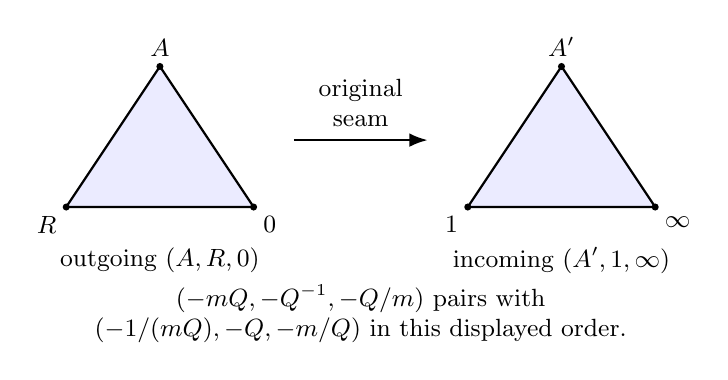
\begin{tikzpicture}[scale=.85,>=Latex,every node/.style={font=\small}]
\coordinate(A) at(0,2.1);\coordinate(R) at(-1.4,0);
\coordinate(Z) at(1.4,0);
\coordinate(B) at(6,2.1);\coordinate(O) at(4.6,0);
\coordinate(I) at(7.4,0);
\fill[blue!8] (A)--(R)--(Z)--cycle;
\fill[blue!8] (B)--(O)--(I)--cycle;
\draw[thick] (A)--(R)--(Z)--cycle;
\draw[thick] (B)--(O)--(I)--cycle;
\foreach \p/\lab/\pos in {A/A/above,R/R/below left,Z/0/below right,B/A'/above,O/1/below left,I/\infty/below right}
 {\fill(\p)circle(1.5pt);\node[\pos]at(\p){$\lab$};}
\draw[->,thick] (2,1)--(4,1);
\node[above,align=center] at(3,1.05){original\\seam};
\node at(0,-.8){outgoing $(A,R,0)$};
\node at(6,-.8){incoming $(A',1,\infty)$};
\node[align=center] at(3,-1.6)
 {$(-mQ,-Q^{-1},-Q/m)$ pairs with\\
  $(-1/(mQ),-Q,-m/Q)$ in this displayed order.};
\end{tikzpicture}

\caption{One pure seam uses the original reversed main-puncture order:
$(A,R,0)$ on the outgoing page is matched with $(A',1,\infty)$
on the incoming page. The three edge ratios multiply to one in
reverse order, so both triangles of the disk side match, including
complex shear. The letters refer to the two local coordinate charts.}
\label{ng:seam-figure}
\end{figure}

\subsection{Positive main meridians and their flags}\label{ng:positive-main-meridians-and-their-flags}

The bipartition signs describe native page coordinates. They are
not extra choices of the knot orientation. At a main boundary
vertex, take the actual small oriented meridian word supplied by
the physical collar. Its local derivative at the displayed ideal
point is \(m\) or \(m^{-1}\), depending on whether that native
meridian is the positive one or its inverse. Transport the word
and its eigenflag together through each face map.

For a main component, choose its orientation at one segment.
The same oriented small meridian propagates by the actual
annular collar conjugacies. The geometric ideal flag propagates
by those same conjugacies, so its chosen eigenvalue stays fixed.
There is no freedom to exchange it after returning around the
component: for generic \(M\), the peripheral longitude commutes
with a nonparabolic meridian and hence preserves both eigenlines.
At \(M=1\) use the analytic limit of this transported flag.
Thus one can record which global component orientation makes
the displayed flag the \(M^{-1}\) source flag. For a knot this
is one global orientation choice, not a separate reset at each
edge. A comparison with an already specified positive
meridian must make this initial choice explicitly.

This identifies the auxiliary products for the pure tree. It makes no identification of the preferred main longitude.

\subsection{The reference map at a parabolic main meridian}\label{ng:parabolic-reference-map}

To fix the sign of the braid collar, we will compare it at \(m=1\)
with the original marked three-point map. In the coordinates above,
the map \((A,R,0)\mapsto(a,\infty,1)\) is represented by
\begin{equation}\label{ng:S6}
 B_{\mathrm o}=
 \begin{pmatrix}(a(A-R)+R)/A&-R\\1&-R\end{pmatrix}.
\end{equation}
Direct substitution gives its three specified values. This reference
map is used in \eqref{ng:S14} to calibrate the physical crossing at
the parabolic main meridian. For the nonparabolic deformation we
construct the braid action on the two puncture generators and
transport their eigenflags and adjacent charts together.

\subsection{A regular matrix implementing the actual positive braid collar}\label{ng:a-regular-matrix-implementing-the-actual-positive-braid-collar}

Let \(a,b\in\mathrm{SL}_2(\mathbb C)\) be the two ordered
puncture meridians in the physical braid frame. They have the
same trace \(M+M^{-1}\). The original positive crossing
convention is

\begin{equation}\label{ng:S8}
(a,b)\longmapsto(a^{-1}ba,a),\qquad P=ba.
\end{equation}

To read the convention, the first strand passes over the second;
its based meridian remains $a$, while moving the other basing path
under it conjugates $b$ to $a^{-1}ba$. The strands exchange their
positions. This is the Wirtinger rule in the original endpoint frame,
and it preserves $ba$, not $ab$.
\begin{figure}[ht]
\centering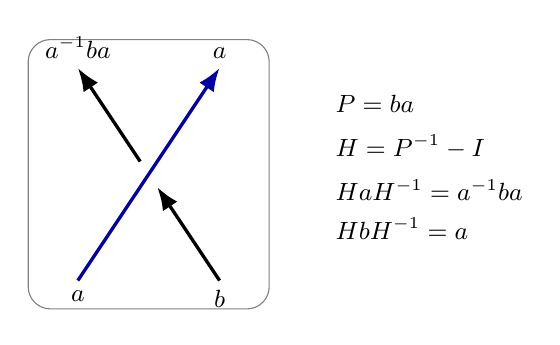
\begin{tikzpicture}[>=Latex,every node/.style={font=\small},scale=.9]
\draw[rounded corners=8pt,gray](-1.7,-.4)rectangle(1.7,3.4);
\draw[very thick,->] (1,0)--(.12,1.32);
\draw[very thick,->] (-.12,1.68)--(-1,3);
\draw[white,line width=6pt] (-1,0)--(1,3);
\draw[blue!65!black,very thick,->](-1,0)--(1,3);
\node[below]at(-1,0){$a$};\node[below]at(1,0){$b$};
\node[above]at(-1,3){$a^{-1}ba$};
\node[above]at(1,3){$a$};
\node[align=left,anchor=west]at(2.5,1.6)
 {$P=ba$\\[5pt]$H=P^{-1}-I$\\[5pt]
  $HaH^{-1}=a^{-1}ba$\\[3pt]$HbH^{-1}=a$};
\end{tikzpicture}

\caption{The retained positive collar and its ordered meridians.
The first strand passes over the second; the output tuple is
$(a^{-1}ba,a)$. The outside disk word $P=ba$ is preserved.
The inverse crossing uses the inverse automorphism.}
\label{ng:hurwitz-figure}
\end{figure}

Put

\begin{equation}\label{ng:S9}
H=P^{-1}-I.
\end{equation}

Near the auxiliary complete lift \(P\), whose trace is \(-2\),
\(\det H=2-\operatorname{tr}P\) is near \(4\).
There is no singular diagonalizing frame.
The Cayley--Hamilton identities for \(a,b\), with their equal
traces, give

\begin{equation}\label{ng:S10}
(P-I)a=b(P-I),\qquad
 (P-I)^2=(\operatorname{tr}P-2)P.
\end{equation}

Consequently \(H\) is projectively \((P-I)^{-1}\), it
commutes with \(P\), and

\begin{equation}\label{ng:S11}
HaH^{-1}=a^{-1}ba,\qquad HbH^{-1}=a.
\end{equation}

This is the exact positive collar rule \eqref{ng:S8}. Its inverse realizes
the negative crossing.

Suppose the selected auxiliary flag has \(P\)-eigenvalue
\(-Q\). The eigenvalue ratio of \(H\) at that flag is

\begin{equation}\label{ng:S12}
\frac{-Q^{-1}-1}{-Q-1}=Q^{-1}.
\end{equation}

Thus composing a pure auxiliary meridian with \(H^\epsilon\)
changes its similarity by \(Q^{-\epsilon}\). It keeps the
disk longitude \(P\) and its chosen flag.

There is an independent matrix calibration against the original
geometric collar. In the local chart set

\begin{equation}\label{ng:S13}
P=m^{-1}W_2^{-1}W_0.
\end{equation}

This is the determinant-one disk word and has selected
eigenvalue \(-Q\). At \(m=1\), for all nearby \(E_0,Q\),
not just at the complete point,

\begin{equation}\label{ng:S14}
S_v^{-1}(P^{-1}-I)=W_0^{-1}B_{\mathrm o}
                        \quad\text{projectively}.
\end{equation}

The right side is the original physical positive-\(R\)
meridian of \cite[Section~5, equations~(5.1)--(5.2)]{Strict}.
That local collar traces the same incoming and outgoing ordered
triangles; only its coordinate normalization differs.
The inverse crossing follows the oppositely signed half-twist path.
Equations \eqref{ng:S8} and \eqref{ng:S14} fix both the braid sign and the actual
copy/collar marking; the sign has not been chosen from a desired
source formula.

\subsection{The full ordered boundary groups in the actual edge chart}\label{ng:the-full-ordered-boundary-groups-in-the-actual-edge-chart}

Let \(N_j=W_{j-1}^{-1}W_j\), with indices modulo four.
Their determinant-one lifts, in the order of the original
equatorial boundary, are

\begin{equation}\label{ng:S14a}
A_g=M^{-3}N_3,\qquad B_g=MN_0,\qquad
 C_g=MN_1,\qquad D_g=MN_2,\qquad
                    A_gB_gC_gD_g=I.
\end{equation}

Each trace is \(M+M^{-1}\). These lifts follow from
\(\det W_0=L,\det W_1=L/m,\det W_2=L/m^2,\det W_3=Lm\).
They include the native loop directions, which need not all be
positive main meridians.

The pure edge returns give the following complete boundary
intertwinings:

\begin{equation}\label{ng:S14b}
\begin{array}{c|c|c|c|c}
 \text{circle}&(a,b)\text{ on the input side}
 &(a',b')\text{ on the output side}&C_0&P=ba=b'a'\\ \hline
 v&(B_g,A_g)&(C_g^{-1},D_g^{-1})&S_v^{-1}&A_gB_g\\
 w&(B_g^{-1},C_g^{-1})&(A_g,D_g)&S_w^{-1}&(B_gC_g)^{-1}.
\end{array}
\end{equation}

Here \(C_0aC_0^{-1}=a'\) and \(C_0bC_0^{-1}=b'\).
For example the first row is equivalent to

\begin{equation}\label{ng:S14c}
S_v C_g S_v^{-1}=B_g^{-1},\qquad
 S_v D_g S_v^{-1}=A_g^{-1}.
\end{equation}

The second is equivalently
\(S_w A_gS_w^{-1}=B_g^{-1}\) and
\(S_w D_gS_w^{-1}=C_g^{-1}\).
These are consequences of the full white/shaded returns;
they may also be checked by direct multiplication of the local
matrices. The product columns agree because
\(D_g^{-1}C_g^{-1}=A_gB_g\) and
\(D_gA_g=(B_gC_g)^{-1}\).

The disk convention \(P=ba\) is therefore explicit at both
ends, including the inversions caused by the turned second
circle. The same table transports under the actual conjugating
frames in a tree; an orientation reversal transports the whole
tuple and its disk word. It does not silently replace \(P\)
by a different boundary product.

For the positive braid put \(H=P^{-1}-I\) in the input
frame. Then \(C_+=C_0H\) satisfies

\begin{equation}\label{ng:S14d}
\begin{aligned}
 C_+aC_+^{-1}&=a'^{-1}b'a',\\
 C_+bC_+^{-1}&=a',\\
 C_+PC_+^{-1}&=P .
\end{aligned}
\end{equation}

For the negative braid use \(H^{-1}\) and the inverse
automorphism. Thus the construction checks both generators of
the actual twice-punctured disk and its outer boundary word;
it is stronger than checking a peripheral similarity or three
traces. Formula \eqref{ng:S14} fixes the positive crossing in the
original physical convention.

\subsection{The opposite-eigenflag qualification}\label{ng:the-opposite-eigenflag-qualification}

Let \(F_a,F_b\) be the two displayed puncture flags, with
eigenvalues \(\lambda_a,\lambda_b\). The natural braid output
flags for \eqref{ng:S8} are

\begin{equation}\label{ng:S15}
(a^{-1}F_b,F_a).
\end{equation}

Their eigenvalues are \((\lambda_b,\lambda_a)\), since
the strands have exchanged positions. By contrast,
\((HF_a,HF_b)\) has eigenvalues
\((\lambda_a,\lambda_b)\) on that same output tuple.
If the selected eigenvalues agree, the two descriptions coincide
by uniqueness of the relevant eigenline. If they differ, use
\(H\) on the opposite input eigenlines to obtain \eqref{ng:S15}.
At a native pure circle the geometric flags on its two main
punctures have opposite selections \(M^{-1},M\).
The qualification is therefore essential.

This identifies the error in an unqualified instruction to
transport both displayed flags by \(H\). The intertwiner is
correct; the displayed decorated triangle needs the accompanying
Weyl change. The two eigenlines coalesce at the parabolic point,
so the complete figure alone cannot distinguish the operations.

\subsection{Representation gluing followed by global decoration}\label{ng:representation-gluing-followed-by-global-decoration}

The following construction keeps that distinction explicit.
First perform the actual collar gluing at the level of
representations; then select the geometric eigenflags on the
resulting original link group.

The half-twist is the actual mapping cylinder of the two-punctured
disk, fixing its outer boundary. Its two boundary generator
tuples are related by \eqref{ng:S8}. If \(C\) is the pure boundary
intertwiner, replacing it by \(CH^\epsilon\), with the side
and composition order fixed by \eqref{ng:S14}, supplies the new
intertwiner. Equation \eqref{ng:S11} verifies the two puncture relations;
\([H,P]=0\) verifies the outer disk-boundary relation. These
are the generators and relation of the twice-punctured disk.
The van Kampen presentation of that actual cut therefore gives
the representation of the reglued exterior. It uses the one
distinguished disk seam at that circle, once.

Apply the operation in every original circle's transported
puncture frame. The other cyclic page seams remain those of
the pure-page construction above. At this stage no assertion is made that the old
pure ideal vertices still provide the correct decoration.

For each resulting main component, choose its actual positive
meridian and its \(M^{-1}\) eigenflag. At a corner whose
native loop is the inverse, take the corresponding \(M\)
eigenflag. Transport these choices by the original paths in the
completed cut. Peripheral commutation makes the choice independent
of a peripheral path. Keep the already selected disk-longitude
flag on each auxiliary circle.

These choices are holomorphic near the complete structure.
For example, for a noncentral matrix
\(\left(\begin{smallmatrix}a&b\\c&d\end{smallmatrix}\right)\)
with \(b\ne0\), an eigenline with prescribed holomorphic
eigenvalue \(\lambda\) is represented by
\((b,\lambda-a)\). The opposite eigenline is obtained by
replacing \(\lambda\) by \(\lambda^{-1}\).
Both approach the unique parabolic flag at the complete point.
A change of coordinate handles a chart with \(b=0\).
The same argument applies to the selected auxiliary eigenvalue
\(-Q\).

Develop the original topological ideal triangulation from these
global flags and the constructed representation. The map of
each triangle is the unique map of its transported ordered
triple. The adjacent white maps are defined from these transported
triples as well, so they carry the same eigenflag choices.
Equivariance gives every edge return. At the complete parameter,
\eqref{ng:S14} and the original collar convention identify the actual odd
development. Its positively oriented tetrahedra therefore remain
positive in a sufficiently small neighborhood of the fixed
finite tree. This is a local decorated representation
construction, not a global completeness assertion for a
nonparabolic main cusp.

The tuple with \(P=ba\) is exactly \eqref{ng:S14b}, transported in the
original physical collar. The positive main loops are chosen
in the completed cut. For the canonical four-segment traversal,
they are \(C_g,B_g^{-1},A_g,D_g^{-1}\) at
\(\infty,0,R,1\), respectively; all four select their geometric
corner with eigenvalue \(M^{-1}\). A reversed physical route
transports both its loop direction and its flag. The preceding
opposite-eigenflag calculation describes the required Weyl change.

At representation level the primitive auxiliary increment is

\begin{equation}\label{ng:S16}
U_v^{\exp}
       =Q_v^{-\epsilon_v}
          \prod_{e\ni v}\frac{Q_v+X_e}{1+Q_vX_e},\qquad
 V_v^{\exp}=Q_v^2.
\end{equation}

It is unchanged by the main-flag redecoration. The exponentiated filling
equation with \(n_v=\epsilon_v-2p_v\) is then

\begin{equation}\label{ng:S17}
\prod_{e\ni v}\frac{Q_v+X_e}{1+Q_vX_e}
                                =Q_v^{n_v}.
\end{equation}

The auxiliary formulas retain the original circle words. The argument does not replace a boundary word by a scalar merely because the local representation has the correct traces. The remaining issue for the local filled germ is rigidity with the primitive logarithmic mark; we establish it next.

\section{The positive anchor and the continued filling mark}
\label{ng:anchor}

We first identify the family at $M=1$ with the original positive
geometric family, including the endpoint of its filling path.
This step does not follow just from agreement at the complete point.

Put $Q=e^{\ii t}$, $P=e^{\ii u}$ with $|t|,|u|\le10^{-2}$,
and write $y=\tan(t/2)$, $z=\tan(u/2)$ and
$k=(1+y^2+z^2)^{-1/2}$, with $k=1$ at zero.
The angular chart of \cite[Section~3, equations~(3.3)--(3.5)]{Circle}
has
\begin{equation}\label{ng:angular-match}
 E=\frac{1+\ii k}{1-\ii k},\qquad
 R=\frac{1+z^2}{2+y^2+z^2},\qquad
 H_0=\frac{1-ky}{1+ky},\quad H_1=\frac{1-kz}{1+kz}.
\end{equation}
At $m=1$, equation \eqref{ng:N16} becomes
\[
 X+X^{-1}=\frac{4-\beta\gamma}{\beta+\gamma+4}
       =\frac{2(y^2+z^2)}{2+y^2+z^2}.
\]
Thus $X=E_0=E$ on the branch through $\ii$.
The first apex is
$(E+Q)/(1+Q)=(1+E)/(1+H_0)$.
Writing $Z_1=(1+E)/(1+H_1)$, the second is
$P(1-E)/(P+1)=RZ_1/(Z_1-(1-R))$.
These are exactly the ordered apices of the angular block.
The four matrices \eqref{ng:N3} specialize projectively to its
four white maps. For example $W_2$ differs from the representative
in \cite[equation~(3.8)]{Circle} only by a scalar.
The pure shaded maps agree because they have the same three ordered
images. Equation \eqref{ng:S14} identifies the odd collar for all
nearby $E,Q$, so it also agrees along this angular family.
The entire marked representation, rather than just its peripheral
trace, is therefore the same one.

For clarity, these formulas are regular throughout the stated angular
bidisk. The elementary Taylor bounds give
$|Q-1|,|P-1|<11/1000$ and
$|\beta-2|,|\gamma-2|<1/9000$.
Indeed $e^r-1\le r/(1-r)$ and
$2(\cosh r-1)\le r^2/(1-r^2)$ for $r=1/100$.
Hence $|X+X^{-1}|<1/16000$; the root through $\ii$ has
$|X-\ii|<1/1000$.
For the last assertion write
$X=A_0/2+\ii\sqrt{1-A_0^2/4}$ with $A_0=X+X^{-1}$,
using the square-root branch at one.
At $m=1$,
$R=(X+X^{-1}+\beta)/(\beta+2)$, so $|R-1/2|<1/1000$.
The apices in \eqref{ng:N5} differ from their complete values by
less than $1/50$. The finite defining vertices therefore stay
distinct, and all displayed denominators stay nonzero.
Moreover
\[
 G|_{m=1}=PQ(\beta+\gamma+4)
              \{E_0^2-(X+X^{-1})E_0+1\}
\]
has a simple root on this bidisk. The change \eqref{ng:N12}
has derivative one in $E_0$ at $m=1$.
Thus the native charts extend holomorphically in $M$ around every
point of the angular family. For a fixed finite tree, compactness of
its charge path supplies finitely many overlapping such charts.
No unspecified complete-point radius is substituted for this path.

Let $\Psi(\boldsymbol\tau)=\sum_{vw}\psi(\tau_v,\tau_w)$ be the
classical angular potential of \cite[equation~(1.3)]{Circle};
its normalization and its derivatives are
\[
 \psi(0,0)=v_{\rm oct}/\pi,\qquad
 \psi_t(t,u)=-\frac1\pi
       \operatorname{arsinh}\bigl(\tan(t/2)\cos(u/2)\bigr).
\]
The actual auxiliary increments in that paper give
\begin{equation}\label{ng:anchor-logs}
 U_v=-2\pi\Psi_{\tau_v}-\ii\epsilon_v\tau_v,\qquad
 V_v=2\ii\tau_v,\qquad Q_v=e^{\ii\tau_v}.
\end{equation}
This is the specialization of \eqref{ng:T3}, with the same
curves and logarithms, since the local maps just matched.
The charge path satisfies
\begin{equation}\label{ng:charge-path}
 \Psi_{\tau_v}+\frac{\ii n_v}{2\pi}\tau_v=\ii c
 \quad\Longleftrightarrow\quad
 U_v+p_vV_v=-2\pi\ii c,\qquad 0\le c\le1.
\end{equation}
The logarithms are continued from $c=0$, not reset to principal
values. The constant on the right records one primitive winding
at $c=1$.

Under either geometric criterion in Theorem~\ref{ng:filled-germ},
\cite[Theorems~1.1 and~7.1]{Circle} constructs this positive
path, identifies the full log-link periods, and proves smooth
completion at $c=1$ on the original filled exterior.
It also proves $\operatorname{Im}\tau_v(c)<0$ for $c>0$.
Consequently $|Q_v|>1$ there, so every filled longitude has
distinct eigenvalues. Intermediate $0<c<1$ has cone angle
$2\pi c$ and generally does not descend to the smooth filled group.
Only the endpoint is used below.

\section{Local rigidity on the retained augmented triangulation}
\label{ng:rigidity}

We give the local rigidity argument with hypotheses that can be checked
on another original positive augmented triangulation as well.
There is no assertion that an arbitrary hyperbolic manifold has the
particular positive triangulation required here.

\begin{proposition}[Marked positive gluing]\label{ng:positive-germ}
Let an oriented ideal triangulation of a specified manifold have $t$
tetrahedra, all with positive shapes, and $c$ torus ends. Retain all
actual face pairings, peripheral paths, developed flags and continuous
edge-log branches. The ends may be incomplete. Suppose the edge
equations hold and all face triples are distinct.
Choose one nonzero primitive peripheral class on each torus.
Its $c$ similarity logarithms are local holomorphic coordinates on
the decorated representation germ modulo simultaneous projective
conjugation. The shape and decorated-representation descriptions are
inverse also over local Artin algebras with this residue point.
\end{proposition}

\subsection{The real row space}
For each positively ordered tetrahedron use
\begin{equation}\label{ng:shape-coordinates}
 u_j=\log z_j,\qquad v_j=-\log(1-z_j),\qquad
 T_j=\frac{\dd v_j}{\dd u_j}=\frac{z_j}{1-z_j},
 \qquad \operatorname{Im}T_j>0 .
\end{equation}
Logarithms continue from the given solution. The original edge and
peripheral equations are affine linear in these logs. Their constants
need not be small.

Here is the rank calculation. The number of global edges is $t$:
coning off the $c$ torus boundaries gives Euler characteristic $c$,
whereas its cell count is $c-e+2t-t$. A linear dependence among edge
rows assigns numbers $\lambda_{ij}$ to the six edges of each
tetrahedron with the three opposite-pair sums equal.
Those equations are equivalent over $\RR$ to
$\lambda_{ij}=s_i+s_j$. For example
$s_0=(\lambda_{01}+\lambda_{02}-\lambda_{12})/2$ and the
other $s_i$ follow; the opposite-sum conditions give the remaining
three edges. The three edge values on a face determine its three
$s_i$ uniquely, so the values descend to one per ideal vertex.
Conversely every such vertex assignment is a dependence.
The assignment is injective, since the three zero endpoint sums
on one triangle force all three vertex values to vanish.
The edge-row space $\mathcal E$ therefore has dimension $t-c$.

We use the actual normal-path identity proved in
\cite[Section~7.1, equations~(7.1)--(7.2)]{Marked}.
It identifies each path row with its developed similarity logarithm
and proves that the row pairing is twice oriented intersection,
up to its fixed coordinate sign. Briefly, the local outgoing-flow
formula is a sum of two-coordinate determinants plus one skew form
on each face. Paired face forms cancel under the orientation-reversing
face identifications. A small normal circle about an edge endpoint
is that edge's incidence row and is null-homologous on the cusp.
Thus $\mathcal E$ is isotropic and orthogonal to every peripheral
row. The $2c$ rows of primitive peripheral bases are independent
in $\mathcal E^\perp/\mathcal E$, because their pairings are
nonzero on each torus and zero between different tori.
Its dimension is $2c$, so those rows form a basis.

The cited calculation uses $(u,v_{\rm old})=(\log z,\log(1-z^{-1}))$.
Here $v_{\rm old}=-u-v+\text{constant}$; the real coordinate
change has determinant $-1$. It reverses the pairing sign but
preserves all ranks and isotropy. Thus the same conclusions hold
for \eqref{ng:shape-coordinates}. No longitude divisibility or
special knot homology assertion is used.

The chosen one-per-torus classes are independent modulo
$\mathcal E$ and pair to zero. Append them to $t-c$ independent
edge rows. The resulting real $t$-row matrix $(A\ B)$ satisfies
\begin{equation}\label{ng:real-rows}
 \operatorname{rank}(A\ B)=t,\qquad
 AB^{\mathsf T}=BA^{\mathsf T}.
\end{equation}
Its kernel is spanned by $(-B^{\mathsf T}y,A^{\mathsf T}y)$ and
is a real Lagrangian space for
$\Omega((a,b),(a',b'))=a\cdot b'-b\cdot a'$.

\subsection{Positive polarization and the actual representation germ}
The selected logarithmic Jacobian is
$J=A+B\diag(T_j)$.
If $Jx=0$, then
$w=(x,\diag(T_j)x)$ and $\overline w$ belong to the
complexified real Lagrangian kernel. But
\begin{equation}\label{ng:polarization}
 \frac{\ii}{2}\Omega(w,\overline w)
              =\sum_j\operatorname{Im}T_j\,|x_j|^2 .
\end{equation}
Its left side is zero, and its right side is positive for $x\ne0$.
Thus $J$ is invertible. Dependent edge rows have compatible affine
constants because the given point satisfies all original equations.
The holomorphic implicit-function theorem proves the asserted
coordinate statement for the shape germ.

This is the actual decorated representation germ. Normalize one
ordered developed triple. The shapes develop successive tetrahedra
across their paired faces by the unique map of three distinct
vertices. An edge return fixes its two distinct endpoints and
has multiplier one by the actual edge equation; hence it is
projectively identity. The dual two-skeleton of the original
triangulation presents its fundamental group. The constructed
face maps therefore give a representation of that group, with
the prescribed peripheral fixed flags and path logarithms.

Conversely a nearby representation $\rho$ with selected peripheral
flags $\xi_v$ develops every ideal vertex $gP_v$ as
$\rho(g)\xi_v$, where $P_v$ is its peripheral subgroup.
This is well defined because $P_v$ fixes $\xi_v$.
The distinct face triples and tetrahedral quadruples remain
distinct nearby. Their cross-ratios recover the shapes; the
face transformations agree on three points, and edge products
telescope. The two constructions are inverse after the same
triple normalization. All denominators are units at the given
point, so they remain inverse over local Artin algebras.
Here an Artin algebra is a finite-dimensional local complex
algebra with nilpotent maximal ideal; it records infinitesimal
as well as ordinary nearby deformations.

At a parabolic peripheral matrix it is essential to retain the
exact eigenvalue character. For
$\left(\begin{smallmatrix}1&1\\0&1\end{smallmatrix}\right)$,
the invariant line generated by $(1,\eta)$ can move when
$\eta^2=0$, but its eigenvalue becomes $1+\eta$.
Fixing the exact eigenvalue one forces $\eta=0$.
In general a unit off-diagonal entry gives the selected eigenvector
$(\mu_{12},\lambda-\mu_{11})$ and the same unique free eigenline.
The similarity logs in the proposition retain that character,
not only the unmarked trace. A separately prescribed determinant-one
lift keeps its central signs on its local sign cover.
This proves Proposition~\ref{ng:positive-germ}.

\section{Filling words and the one-dimensional geometric germ}
\label{ng:filling-germ-proof}

At the augmented complete structure choose the main meridian and
the auxiliary longitudes in Proposition~\ref{ng:positive-germ}.
Their logarithms are $-2\log M$ and $2\log Q_v$ in our selected
flags. The explicitly constructed family has these very
coordinates. It therefore exhausts the nearby decorated
augmented representation germ. This completes the local assertion
of Theorem~\ref{ng:representation}. The continuation and positive
anchor in Section~\ref{ng:anchor} prove its endpoint assertion.

Now let $\rho_*$ be a positive primitive filled endpoint as in
Theorem~\ref{ng:filled-germ}. Use the original augmented
triangulation at this endpoint. Its auxiliary ends are incomplete;
the proof of Proposition~\ref{ng:positive-germ} did not require
their completeness or the faithfulness of the augmented representation.
Choose the main meridian and the original slopes
$\sigma_v=\mu_v+p_v\lambda_v$ as its peripheral coordinates.
Each is a primitive nonzero class on a different torus.
Their log rows are real and satisfy exactly the hypotheses of
the proposition. Fixing the $R$ auxiliary slope logs leaves a
smooth one-dimensional shape and decorated representation germ.

We must still identify this condition with the filled group.
A slope word commutes projectively with the auxiliary longitude.
The latter has distinct eigenvalues by hypothesis. Choose a local
representative of the slope whose residue is identity. If its
commutator with the longitude has scalar $c_0$, determinants give
$c_0^2=1$, while $c_0\equiv1$ at the residue point.
Because $c_0+1$ is a unit, $c_0=1$, also over local Artin algebras.
The longitude eigenspaces split the rank-two module because their
eigenvalue difference is a unit. Strict commutation kills both
off-diagonal entries of the slope in that basis.
Equation \eqref{ng:A2} gives eigenvalue ratio one, so the slope
matrix is scalar and hence projectively identity.
This normalization does not reset the signs of a separately
retained determinant-one group lift.

Conversely, a nearby representation of the filled group pulls
back to one whose slopes are projectively identity.
On the continued branch at $\rho_*$ their logarithms are precisely
$-2\pi\ii$, not another multiple of $2\pi\ii$.
The auxiliary eigenflags are uniquely selected by the longitude
branches. At the main cusp retain the exact eigenvalue $M^{-1}$;
the formula for its eigenvector in the preceding proof remains
regular at its noncentral parabolic basepoint.
Thus filled representations and the fixed-slope decorated shape
germ are the same local object, modulo simultaneous conjugation.
Its coordinate is $\log M$, since the main similarity logarithm
on that line is $-2\log M$, a nonzero scalar multiple.

For the tree endpoints, Section~\ref{ng:anchor} supplied the
original smooth metric holonomy and the nonunit auxiliary
longitudes. This proves Theorem~\ref{ng:filled-germ}, without
assuming rigidity from a new positive triangulation of the filled
manifold.

\begin{corollary}[Identification of an independently constructed branch]
\label{ng:branch-identification}
Suppose another holomorphic construction reconstructs the same
original augmented representation at this positive endpoint,
keeps its main eigenflag and primitive logarithmic slope words,
and satisfies \eqref{ng:A2} nearby with the same variable $M$.
Its local representation branch is the geometric meridian germ
of Theorem~\ref{ng:filled-germ}. This holds also for infinitesimal
branches with the exact marked characters retained.
\end{corollary}
\begin{proof}
Both branches lie in the same decorated filled germ, and $\log M$
is a local coordinate on it, including over local Artin algebras.
\end{proof}

In a stationary-source application, nondegeneracy of that source
critical point is one way to supply the independent holomorphic
branch in the corollary. It is not a premise of the geometric
construction or a consequence of a volume derivative. The
preferred main longitude, its framing monomial and a quantum
annihilator remain separate identifications.

\section{Finite verification and scope}\label{ng:scope}

The accompanying \texttt{check.py} replays exact rational identities
for the local face maps, all six edge returns, the meridian wire
change, both seam tables, the character matrices and their
auxiliary transports. It checks the Hurwitz action and its
eigenflag qualification and the elementary polarization identity.
It includes incorrect fixed-white and eigenflag alternatives as
negative controls. With \texttt{--output} it writes a source-hashed
JSON record only after all checks finish and the inputs are
verified unchanged.

These finite identities support the displayed algebra. They do
not prove the inverse-cut topology, positive metric completion,
the full gluing-row rank theorem or the analytic inverse-function
theorem. The paper supplies its own arguments or exact named
imports for those steps. In particular, neither an exponentiated
slope equation nor a character trace calculation is substituted
for a marked group representation or a smooth filling.

The method sits within the classical deformation and peripheral
framework of Neumann--Zagier \cite{NZ}. Our actual row convention
and its geometric meaning are supplied by the direct calculation
in \cite{Marked}; no unspecified rigidity theorem is imported.
The statements here concern the literal ordered trees and the
explicitly stated general positive-germ lemma, not arbitrary
matching graphs or arbitrary incomplete hyperbolic structures.

\begin{thebibliography}{9}
\bibitem{Circle}
\emph{Positive octahedra and primitive fillings for trees of crossing circles},
companion paper, Proposition~2.1, Lemma~3.1 and
Theorems~1.1 and~7.1.
\href{https://sashakolpakov.github.io/murakamis_dream/papers/circle-tree-geometry.pdf}
{Companion PDF}.

\bibitem{Strict}
\emph{Marked geometry of strict Conway compositions},
companion paper, Section~5, equations~(5.1)--(5.2).
\href{https://sashakolpakov.github.io/murakamis_dream/papers/strict-conway-geometry.pdf}
{Companion PDF}.

\bibitem{Marked}
\emph{Circle patterns and primitive fillings of augmented links},
companion paper, Section~7.1, equations~(7.1)--(7.2).
\href{https://sashakolpakov.github.io/murakamis_dream/papers/marked-fillings.pdf}
{Companion PDF}.

\bibitem{NZ}
W.~D.~Neumann and D.~Zagier,
Volumes of hyperbolic three-manifolds,
\emph{Topology} \textbf{24} (1985), 307--332.
\href{https://doi.org/10.1016/0040-9383(85)90004-7}
{doi:10.1016/0040-9383(85)90004-7}.
\end{thebibliography}

\end{document}
